\documentclass{article}
\usepackage{graphicx}
\usepackage{amsmath}
\usepackage{hyperref}
\usepackage[utf8] {inputenc}
\usepackage{polski}
\usepackage{geometry}
\usepackage{listings}
\usepackage{xcolor}

\geometry{
    a4paper,
    total={170mm,257mm},
    left=40mm,
    right=40mm,
    top=20mm,
    bottom=20mm,
}

\usepackage[utf8]{inputenc} % Obsługa polskich znaków
\usepackage[T1]{fontenc} % Kodowanie fontu dla polskich znaków
\usepackage{listings} % Pakiet do wstawiania kodu źródłowego
\usepackage{xcolor} % Pakiet do zarządzania kolorami
\definecolor{fiolet}{rgb}{0.498, 0.318, 0.961}
\definecolor{zielony}{rgb}{0.094, 0.6, 0.078}

\lstset{
    language=Python,
    basicstyle=\ttfamily\small, % Podstawowy styl czcionki
    keywordstyle=\color{fiolet}, % Kolor słów kluczowych
    stringstyle=\color{zielony}, % Kolor ciągów znaków
    morekeywords={srednia_ocen}, % Dodatkowe słowa kluczowe
    showstringspaces=false, % Nie pokazuj odstępów w ciągach znaków
    breaklines=true, % Automatyczne łamanie długich linii
    numbers=left, % Numeracja linii po lewej stronie
    numberstyle=\small\color{gray}, % Styl numerów linii
    frame=single, % Ramka wokół kodu
    extendedchars=true, % Włączenie obsługi rozszerzonych znaków (w tym polskich)
    literate=%
        {ą}{{\k{a}}}1
        {ć}{{\'c}}1
        {ę}{{\k{e}}}1
        {ł}{{\l{}}}1
        {ń}{{\'n}}1
        {ó}{{\'o}}1
        {ś}{{\'s}}1
        {ź}{{\'z}}1
        {ż}{{\.z}}1
        {Ą}{{\k{A}}}1
        {Ć}{{\'C}}1
        {Ę}{{\k{E}}}1
        {Ł}{{\L{}}}1
        {Ń}{{\'N}}1
        {Ó}{{\'O}}1
        {Ś}{{\'S}}1
        {Ź}{{\'Z}}1
        {Ż}{{\.Z}}1,
}

\begin{document}
\title{\textbf{\textit{Analiza danych - Python}}}
\author{\textit{Skład: Robert Baca, Arkadiusz Bodziony, Wiktor Ciskał, Mikołaj Śnieżko}}
\date{Praca wykonywana w okresie II kwartału roku 2024}
\maketitle

\vspace{1cm}
\section{Wprowadzenie}
W ramach tego projektu zajmujemy się analizą danych szkolnych, w tym ocen i frekwencji uczniów z różnych regionów. Wykonamy różne analizy statystyczne i przedstawimy je za pomocą wykresów.

\section{Przygotowanie danych}
\begin{itemize}
    \item Struktura pliku danych: \texttt{address, absences, Mjob, Fjob, math\_grade}
    \item Kolumny \texttt{address} zawierają wartości \texttt{U} (miejski) i \texttt{R} (wiejski).
    \item Kolumna \texttt{absences} zawiera liczbę nieobecności ucznia.
    \item Kolumny \texttt{Mjob} i \texttt{Fjob} oznaczają zawody matki i ojca.
    \item Kolumna \texttt{math\_grade} oznacza końcową ocenę z matematyki w skali 0-20.
\end{itemize}

\section{Średnie oceny}
\begin{lstlisting}[language=Python]
def srednia_ocen(adr, oceny):
    licznik_w = 0
    licznik_m = 0
    sum_wiejski = 0
    sum_miejski = 0

    for i, j in zip(oceny, adr):
        if j == 'r':
            sum_wiejski += i
            licznik_w += 1
        elif j == 'u':
            sum_miejski += i
            licznik_m += 1

    srednia_wiejski = sum_wiejski / licznik_w if licznik_w != 0 else 0
    srednia_miejski = sum_miejski / licznik_m if licznik_m != 0 else 0

    return round(srednia_miejski, 2), round(srednia_wiejski, 2)
\end{lstlisting}

\begin{flushleft}
Średnia ocen dla miasta wynosi \texttt{10.69}, a dla wsi \texttt{9.47}. Z tego wynika, że uczniowe z miasta mają statystycznie lepsze stopnie w szkole.
\end{flushleft}
\vspace{3cm}

\section{Mediana ocen}
\begin{lstlisting}[language=Python]
def mediana_ocen(adr, oceny):
    wiejski = [i for i, j in zip(oceny, adr) if j == 'r']
    miejski = [i for i, j in zip(oceny, adr) if j == 'u']
    
    return median(oceny), median(miejski), median(wiejski)
\end{lstlisting}

\begin{flushleft}
Mediana wszystkich ocen wynosi \texttt{11.0}, dla miasta \texttt{11.0}, dla wsi \texttt{11.0}. Zatem mediana ocen jest identyczna dla obu kategorii.
\end{flushleft}

\section{Odchylenie standardowe}
\begin{lstlisting}[language=Python]
def sigma(x):
    return sqrt((sum([(i-mean(x))**2 for i in x])/len(x)))
\end{lstlisting}
\begin{lstlisting}[language=Python]
def odchyl_std(adr, oceny):
    wiejski = [i for i, j in zip(oceny, adr) if j == 'r']
    miejski = [i for i, j in zip(oceny, adr) if j == 'u']
    
    return sigma(oceny), sigma(miejski), sigma(wiejski)
\end{lstlisting}

\begin{flushleft}
Odchylenie standardowe wszystkich ocen wynosi \texttt{4.58}, dla miasta \texttt{11.0}, dla wsi \texttt{10.0}. Te pomiary mogą nas naprowadzić na tezę, że oceny uczniów z miasta osiągają większe amplitudy.
\end{flushleft}

\section{Moda}
\begin{lstlisting}[language=Python]
def obliczanie_mody(adr, oceny):
    wiejski = [i for i, j in zip(oceny, adr) if j == 'r']
    miejski = [i for i, j in zip(oceny, adr) if j == 'u']
    
    return moda(oceny), moda(miejski), moda(wiejski)
\end{lstlisting}
\begin{lstlisting}[language=Python]
def moda(liczby):
    najczesciej = {}
    for i in liczby:
        if i in najczesciej:
            najczesciej[i] += 1
        else:
            najczesciej[i] = 1
            
    max_licznik = 0
    najczesciej_liczba = 0
    
    for wartosc, licznik in najczesciej.items():
        if licznik > max_licznik:
            max_licznik = licznik
            najczesciej_liczba = wartosc
    
    return najczesciej_liczba
\end{lstlisting}

\begin{flushleft}
Moda dla wszystkich ocen wynosi \texttt{10}, dla miasta \texttt{10}, dla wsi \texttt{10}. Podobnie jak w przypadku mediany, moda jest równa w obu grupach.
\end{flushleft}
\vspace{2cm}

\section{Regresja liniowa i współczynnik R$^2$}
\begin{lstlisting}[language=Python]
def korelacja_regresja_r2(nobec, oceny):
    return korelacja(nobec, oceny), reg_liniowa(nobec, oceny), r2(nobec, oceny)
\end{lstlisting}
\begin{lstlisting}[language=Python]
def korelacja(x, y):
    return sum([(i-mean(x))*(j-mean(y)) for i, j in zip(x, y)])/
    sqrt(sum([(i-mean(x))**2 for i in x]) * sum([(i-mean(y))**2 for i in y]))
\end{lstlisting}
\begin{lstlisting}[language=Python]
def reg_liniowa(x, y):
    a1 = sum([(i-mean(x))*(j-mean(y)) for i, j in zip(x, y)])/
    sum([(i-mean(x))**2 for i in x])
    a0 = mean(y-(a1*mean(x)))
    return f'{round(a0, 2)}x + {round(a1, 2)}'
\end{lstlisting}
\begin{lstlisting}[language=Python]
def r2(x, y):
    return 1-(sum((i-mean(y))**2 for i in y)/sum((j-i)**2
    for i, j in zip(x, y)))
\end{lstlisting}

\begin{flushleft}
Wspołczynnik korelacji między nieobecnością a oceną wynosi \texttt{0.03}, regresja liniowa \texttt{10.3x + 0.02}, a współczynnik R$^2$ jest równy \texttt{0.08}. Korelacja osiąga umiarkową wartość, więc oceny niekoniecznie są powiązane z frekwencją, jednak nie można uznać tego powiązania za nieistniejące.
\end{flushleft}

\section{Przewidywanie punktów}
\begin{lstlisting}[language=Python]
def punkty_predykcja(nieobecnosci, grupy):
    liczba_zajec = 75
    punkty = []
    for liczba_nieobecnosci, grupa in zip(nieobecnosci, grupy):
        liczba_obecnosci = (liczba_zajec - liczba_nieobecnosci)
        punkty_obecnosci = liczba_obecnosci * 5
        if liczba_nieobecnosci == 0:
            punkty_obecnosci += 35
        if grupa == 'r':
            punkty_obecnosci += 2 * liczba_obecnosci
        punkty.append(punkty_obecnosci)

    return punkty
\end{lstlisting}

\begin{flushleft}
Punkty za obecności zostały przedstawione na wykresie w sekcji 'Wizualizacje'. Wypisywanie całej listy, zajęłoby sporo przestrzeni, a nie są to dane niezbędne. Zamieszczone jednak zostaną pierwsze 10 wyników: [345, 497, 325, 365, 355, 325, 410, 345, 410, 410].
\end{flushleft}
\vspace{7cm}

\section{Wizualizacje}

\subsection{Histogram ocen}
\begin{lstlisting}[language=Python]
def histogram_ocen(oceny):
    plt.hist(oceny, bins=20, edgecolor='black', color='orange')
    plt.xlabel('Oceny')
    plt.ylabel('Liczba uczniów')
    plt.title('Histogram ocen')
    plt.show()
\end{lstlisting}
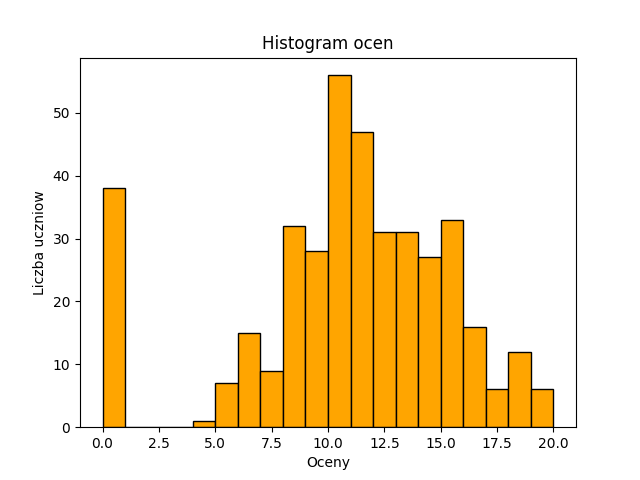
\includegraphics[width=\textwidth]{histogram_ocen.png}
\textbf{Krótki wniosek:} Zdecydowana większość uczniów na koniec roku otrzymała oceny w przedziale [10-12]. Są to wyniki graniczące z warunkami zaliczenia, więc stwierdzić można, że przeważającą grupą uczniów są uczniowe przeciętni. Jednak warto zauważyć, jaka dysproporcja istnieje między ocenami 0, a [17-20]. Prawdpobodnie wynika to z faktu, że oceny 0 wystawiane mogły być za nieoddane projekty, natomiast najwyższe stopnie, otrzymali jedynie wybitni uczniowie. Tezę o ocenach zerowych potwierdzić może brak uczniów w przedziale [1-4].
\vspace{15cm}

\subsection{Histogram punktów}
\begin{lstlisting}[language=Python]
def histogram_punktow(oceny):
    plt.hist(oceny, bins=20, edgecolor='black', color='gold')
    plt.xlabel('Punkty')
    plt.ylabel('Liczba uczniów')
    plt.title('Histogram punktów')
    plt.show()
\end{lstlisting}
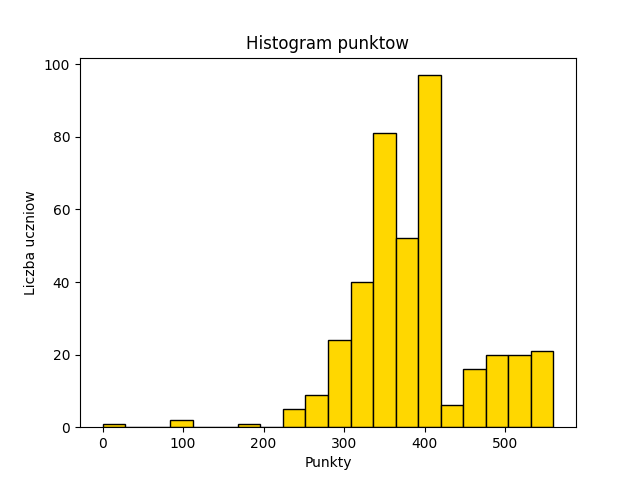
\includegraphics[width=\textwidth]{histogram_punktow.png}
\textbf{Krótki wniosek:} Z wykresu odczytać można, że przeważającym przedziałem jest [330-425]. Wynika to z danych otrzymanych ze szkoły oraz wzoru na wyliczenie przewidywanych punktów. Wzór: liczba obecności*5 + dodatkowe 2 za każdą obecność dla uczniów ze wsi. Większość uczniów opuściło jedynie kilka zajęć, co można odczytać z wykresu. Nieliczni nie opuścili żadnych zajęć, a osób, które nie pojawiły się wcale było bardzo mało.
\vspace{15cm}

\subsection{Udział grup w klasie}
\begin{lstlisting}[language=Python]
def udzial_grup(oceny, adr):
    wiejski = [i for i, j in zip(oceny, adr) if j == 'r']
    miejski = [i for i, j in zip(oceny, adr) if j == 'u']
    
    plt.pie([len(wiejski)/len(oceny), len(miejski)/len(oceny)], labels=
    ['obszar wiejski', 'obszar miejski'], autopct='%0.1f%%', colors=['lime', 'red'])
    plt.legend(['obszar wiejski', 'obszar miejski'], edgecolor='black', loc='upper left')
    plt.axis('equal')
    plt.title('% udziału grup w klasie')
    plt.show()
\end{lstlisting}
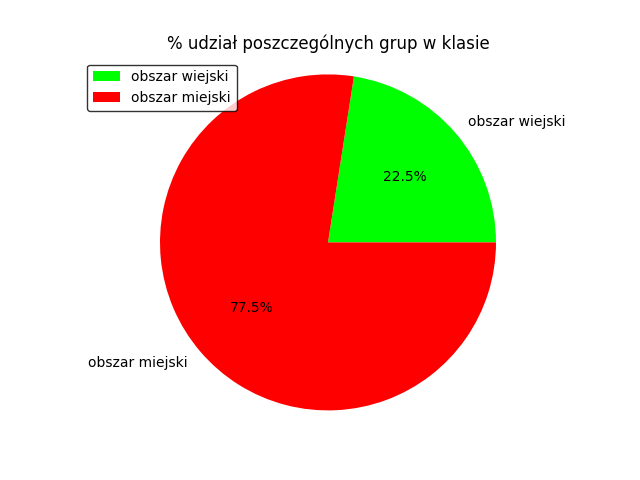
\includegraphics[width=\textwidth]{kolowy.png}
\textbf{Krótki wniosek:} W przypadku tego wykresu, ciężko o jakiekolwiek wnioski poza tymi oczywistymi. Ponad 3/4 uczniów z badanej szkoły zamieszkuje tereny miejskie. 
\vspace{15cm}

\subsection{Wykres punktowy ocen uczniów z obu grup}
\begin{lstlisting}[language=Python]
def punktowy(oceny, adr, nobec):
    o_wiejski = [i for i, j in zip(oceny, adr) if j == 'r']
    o_miejski = [i for i, j in zip(oceny, adr) if j == 'u']
    
    n_wiejski = [i for i, j in zip(nobec, adr) if j == 'r']
    n_miejski = [i for i, j in zip(nobec, adr) if j == 'u']
    
    plt.scatter(o_wiejski, n_wiejski, color='lime')
    plt.scatter(o_miejski, n_miejski, color='red')
    
    plt.title('Punktowy wykres ocen dla dwóch grup')
    plt.ylabel('Nieobecności')
    plt.xlabel('Oceny')
    plt.legend(['Wieś', 'Miasto'], edgecolor='black')
    plt.show()
\end{lstlisting}
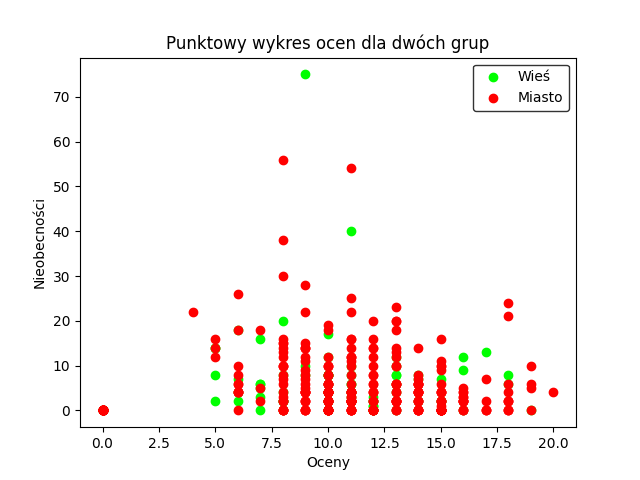
\includegraphics[width=\textwidth]{punktowy_grupy.png}
\textbf{Krótki wniosek:} Ten wykres może być nieco niezrozumiały na pierwszy rzut oka, dlatego spieszymy z pomocą. Zobrazowane tutaj są oceny w skali liczby nieobecności. Widać, że oceny nie są w dużym stopniu skolerowane z ocenami, dane są dość chaotyczne i niepowiązane. Możemy stwierdzić, że pewna korelacja istnieje, jednak zdecydowanie nie jest ona duża. Zdecydowana większość uczniów, była nieobecnych [0-20] razy i osiągają oni oceny [7-13]. Zauważyć możemy, że stosunkowo bardziej odstającymi w obie strony są uczniowie ze wsi, którzy pomimo niewielu nieobecności osiągają stosunkowo niskie i stosunkowo wysokie stopnie. Jednak, prawdodpobnie wynika to z próbki, która jest znacznie mniejsza od studentów z miasta.
\vspace{15cm}

\subsection{Wykres przewidywanych punktów uczniów z obu grup}
\begin{lstlisting}[language=Python]
def wykres_punktowy_predykcji(predykcja, grupa):
    punkty_wsi = [predykcja[i] for i in range(len(predykcja)) if grupa[i] == 'r']
    punkty_miasta = [predykcja[i] for i in range(len(predykcja)) if grupa[i] == 'u']

    plt.scatter(punkty_miasta, [i for i in range(len(punkty_miasta))], color='blue', 
    label='Miasto')
    plt.scatter(punkty_wsi, [i for i in range(len(punkty_wsi))], color='green',
    label='Wieś')

    plt.xlabel('Przewidziane punkty')
    plt.ylabel('ID ucznia')
    plt.title('Przewidziane punkty dla uczniów')
    plt.legend(edgecolor='black')
    plt.show()
\end{lstlisting}
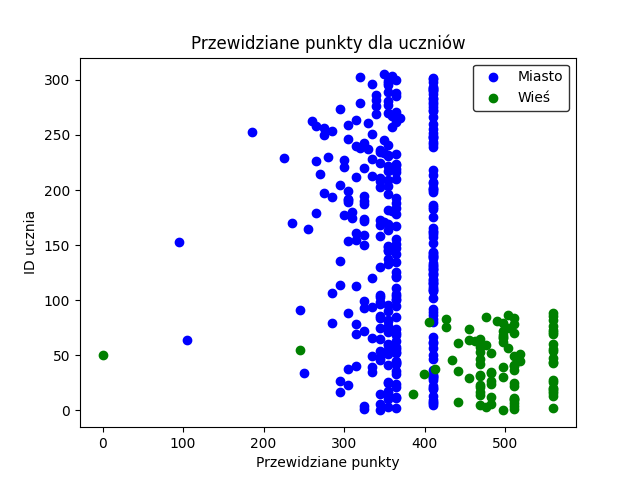
\includegraphics[width=\textwidth]{punkty_przewidziane.png}
\textbf{Krótki wniosek:} Ten wykres również może wydawać się niezrozumiały, jednak ponownie - spokojnie, zaraz będzie on klarowniejszy. Patrząc na legendę, widzimy jakie punkty, co oznaczają. Jest to wykres przedstawiający wszystkich uczniów oraz ich punkty za frekwencję. Widać, że najwięcej uczniów osiągnie ok. 410 punktów. Bliżej maksymalnej wartości są uczniowe ze wsi, co jest dość oczywiste, biorąc pod uwagę nasz wzór na przewidywane punkty. Nie licząc pojedynczych przypadków, widzimy, że uczniowie ze wsi, pojawią się w placówce podobną liczbę razy, jednakże trzeba wziąc poprawkę na to, że mają znacznie cięższy dojazd.
\vspace{15cm}

\subsection{Zawody wsród rodziców uczniów}
\begin{lstlisting}[language=Python]
def zawody_rodzicow(m_zawod, o_zawod):
    job_counts_mother = {}
    job_counts_father = {}

    for job in m_zawod:
        if job not in job_counts_mother:
            job_counts_mother[job] = 0
        job_counts_mother[job] += 1

    for job in o_zawod:
        if job not in job_counts_father:
            job_counts_father[job] = 0
        job_counts_father[job] += 1

    jobs = list(set(m_zawod + o_zawod))
    counts_mother = [job_counts_mother.get(job, 0) for job in jobs]
    counts_father = [job_counts_father.get(job, 0) for job in jobs]

    x = range(len(jobs))
    width = 0.4

    plt.figure(figsize=(12, 6))
    plt.bar(x, counts_mother, width=width, label='Matka', align='center', color='violet', edgecolor='black')
    plt.bar([p + width for p in x], counts_father, width=width, label='Ojciec', align='center', color='coral', edgecolor='black')

    plt.xlabel('Zawód', fontsize=14)
    plt.ylabel('Liczba wystąpień', fontsize=14)
    plt.title('Dominujące zawody rodziców uczniów', fontsize=16)
    plt.xticks([p + width / 2 for p in x], jobs, rotation=45, fontsize=12)
    plt.legend(fontsize=15, edgecolor='black')
    plt.tight_layout()
    plt.show()

    return job_counts_mother, job_counts_father
\end{lstlisting}
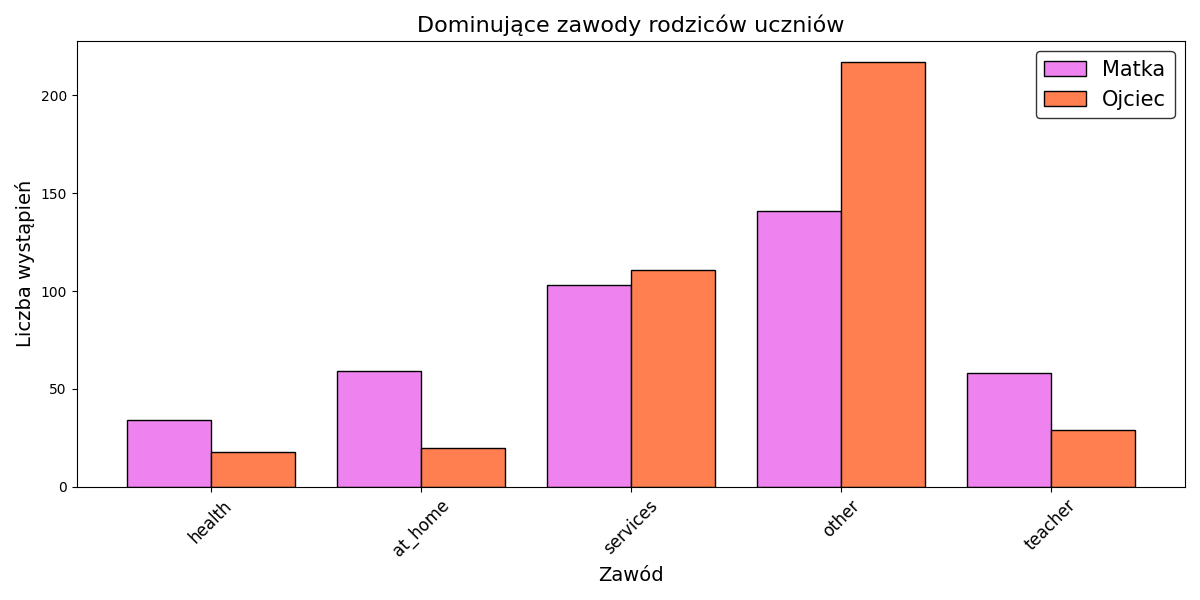
\includegraphics[width=\textwidth]{zawody_rodzicow.png}
\textbf{Krótki wniosek:} Na powyższym wykresie, widzimy liczbę wystąpień każdego z podanych zawodów, obu rodziców uczniów badanej placówki. Widzimy, że przeważającym zawodem (szczególnie wsród ojców) jest 'other', jest dość zrozumiałe, ze względu na to, że do tej grupy wchodzą wszystkie niewymienione w pliku specjalizacje, naturalnym następstwem tego faktu, jest że to matki dominują w pozostałych zawodach (poza usługami).

\section{Wnioski}
\textbf{Podsumowanie wyników analizy i obserwacji.}
\subsection{Oceny i frekwencja:}
\begin{itemize}
    \item Wydaje się, że uczniowie zamieszkujący obszary miejskie odnoszą lepsze sukcesy szkolne w porównaniu do swoich kolegów z obszarów wiejskich. Statystyczna analiza ujawniła, że średnie oceny dla uczniów miejskich wynoszą \texttt{10.69}, podczas gdy dla uczniów wiejskich jest to \texttt{9.47}.
    \item Istnieje również pewna korelacja między frekwencją a wynikami w nauce, choć nie jest ona jednoznaczna. Współczynnik korelacji wynoszący \texttt{0.03} sugeruje, że większa frekwencja może mieć korzystny wpływ na wyniki edukacyjne.
\end{itemize}
\subsection{Rozkład ocen i punktów:}
\begin{itemize}
    \item Analiza rozkładu ocen wykazała, że większość uczniów otrzymuje oceny w przedziale \texttt{[10-12]}, co sugeruje, że są to przeważnie oceny średnie. Interesującą obserwacją jest również znaczna różnica między liczbą ocen zerowych a ocenami w górnym zakresie skali.
    \item Jeśli chodzi o punkty za obecność, większość uczniów zdaje się osiągać około \texttt{410} punktów. Warto zauważyć, że uczniowie z obszarów wiejskich zdają się osiągać nieco więcej punktów niż uczniowie z obszarów miejskich.
\end{itemize}
\subsection{Zawody rodziców uczniów:}
\begin{itemize}
    \item Dominującym zawodem zarówno matek, jak i ojców uczniów jest kategoria "other". Jednakże, gdy rozważymy specjalizacje matki i ojca osobno, obserwujemy pewne różnice. Przykładowo, matki częściej pracują w zawodach związanych z edukacją i opieką zdrowotną, podczas gdy ojcowie częściej pracują w innych branżach.
\end{itemize}
\end{document}
